\section{Systems description} \label{sec:system}

In this section we describe the stance\&gender detection systems. Organizing the system by modules, it can be divided in two blocks: text pre-preprocessing (\Cref{subsec:preprocessing}) and classification model (\Cref{subsec:classificationModel}). 


\subsection{Text pre-processing} \label{subsec:preprocessing}
Regarding the text pre-preprocessing, has to be mentioned that the corpus under observation can not be treated as proper written language, because computer-mediated communication (CMC) is highly informal, affecting diamesic\footnote{The variation in a language across medium of communication (e.g. Spanish over the phone versus Spanish over email)} variation with creation of new items supposed to pertain lexicon and graphematic domains \cite{bazzanella2011oscillazioni,cerruti2013netspeak}.
Therefore, our pre-processing follows two approaches: classic and microblogging related.
As classic aproach we used stemming (i.e., ST), stopwords (i.e., SW) and punctuation removal (i.e., PR).
For microblogging approach we focus our attention over the following items:
\begin{enumerate*}
\item mentions (i.e., MT),
\item smiley (i.e., SM),
\item emoji (i.e., EM),
\item hashtags (i.e., HT),
\item numbers (i.e., NUM),
\item URL (i.e., URL)
\item and Tweeter reserve-word as RT and FAV (i.e., RW).
\end{enumerate*}
For each of these items we leave the possibility to be removed or substituted by constant string.

In relation to above approaches we implement them using the following tools:
\begin{enumerate*}
\item NLTK \cite{nltk} and 
\item Preprocessor\footnote{Preprocessor is a preprocessing library for tweet data written in Python, https://github.com/s/preprocessor}.
\end{enumerate*}



\subsection{Classification models} \label{subsec:classificationModel}
Following, we describe the neural models used for the classification module. Before introducing the models we describe the specific text representation used as input layer \Cref{subsubsec:representation} (i.e., sentence-matrix).

\subsubsection{Text representation} \label{subsubsec:representation}
To represent the text we used word embeddings as described by \cite{bojanowski2016enriching}, where \emph{words} are represented as vectors of real number with fixed dimension $|v|$.
In this way a whole sentence $s$, with length $|s|$ its number of word, is represented as a \emph{sentence-matrix} $M$ of dimension $|M| = |s| \times |v|$. $|M|$ has to be fixed a priori, therefore $|s|$ and $|v|$ have to be estimated. $|v|$ was fixed to 300 following \cite{bojanowski2016enriching}. $|s|$ was estimated analyzing \cref{tab:tweet}, in details we decided to fix it as the sum of average length plus the standard deviation (i.e. $|s| = 17$ for both language), with this choice input sentences longer than $|s|$ are truncated, while shorter ones are padded with null vectors (i.e., a vector of all zeros).

Choosing words as elements to be mapped by the embedding function, raise some challenge over the function estimation related to data availability. In our case the available corpus is very small and estimated embeddings could lead to low performance.
To solve this problem, we decided to used a pre-trained embeddings estimated over Wikipedia using a particular approach called \emph{fastText} \cite{bojanowski2016enriching}.


\subsubsection{Convolutional Neural Network.}
Convolutional Neural Networks (CNN) are considered state of the art in many text classification problem. Therefore, we decide to use them in a simple architecture composed by a convolutional layer, followed by a \emph{Global Max Pooling} layer and two dense layers.

\subsubsection{Dilated KIM.}
This model is our new topology of CNN. It can be seen as an extension of Kim's model \cite{kim2014convolutional} using the dilation ideas from computer graphics field \cite{yu2015multi}.

The original Kim's model is a particular CNN where the convolutional layer has multiple filter widths and feature maps.
The complete architecture is illustrated in \Cref{fig:kim}, here the input layer (i.e., sentence-matrix) is processed in a convolutional layer of multiple filters with different width, each of these results are fed into \emph{Max Pooling} layers and finally the concatenation of them (previously flatten to be dimensional coherent) is projected into a dense layer.
Our extension is to use a dilated filters in combination with normal ones, the intuition is that normal filter capture \emph{adjacent words} features, while dilated one are able to capture relations between \emph{non adjacent words}.
This behaviour can't be achieved by the original Kim's model, because, even though the filters size can be changed, they will capture only features from adjacent words.

Regarding the architectural references in \cite{kim2014convolutional}, the filter's number $|f|$ and their dimension $(k,d)$, where $k$ is the kernel size and $d$ the dilation's unit, was optimized leading to the following results: $|f| = 5, f_1 = (2\times2,0), f_2 = (2\times2,3), f_3 = (3\times3,1), f_4 = (5\times5,1), f_5 = (7\times7,1)$.

\begin{figure}[h]
\footnotesize
\centering
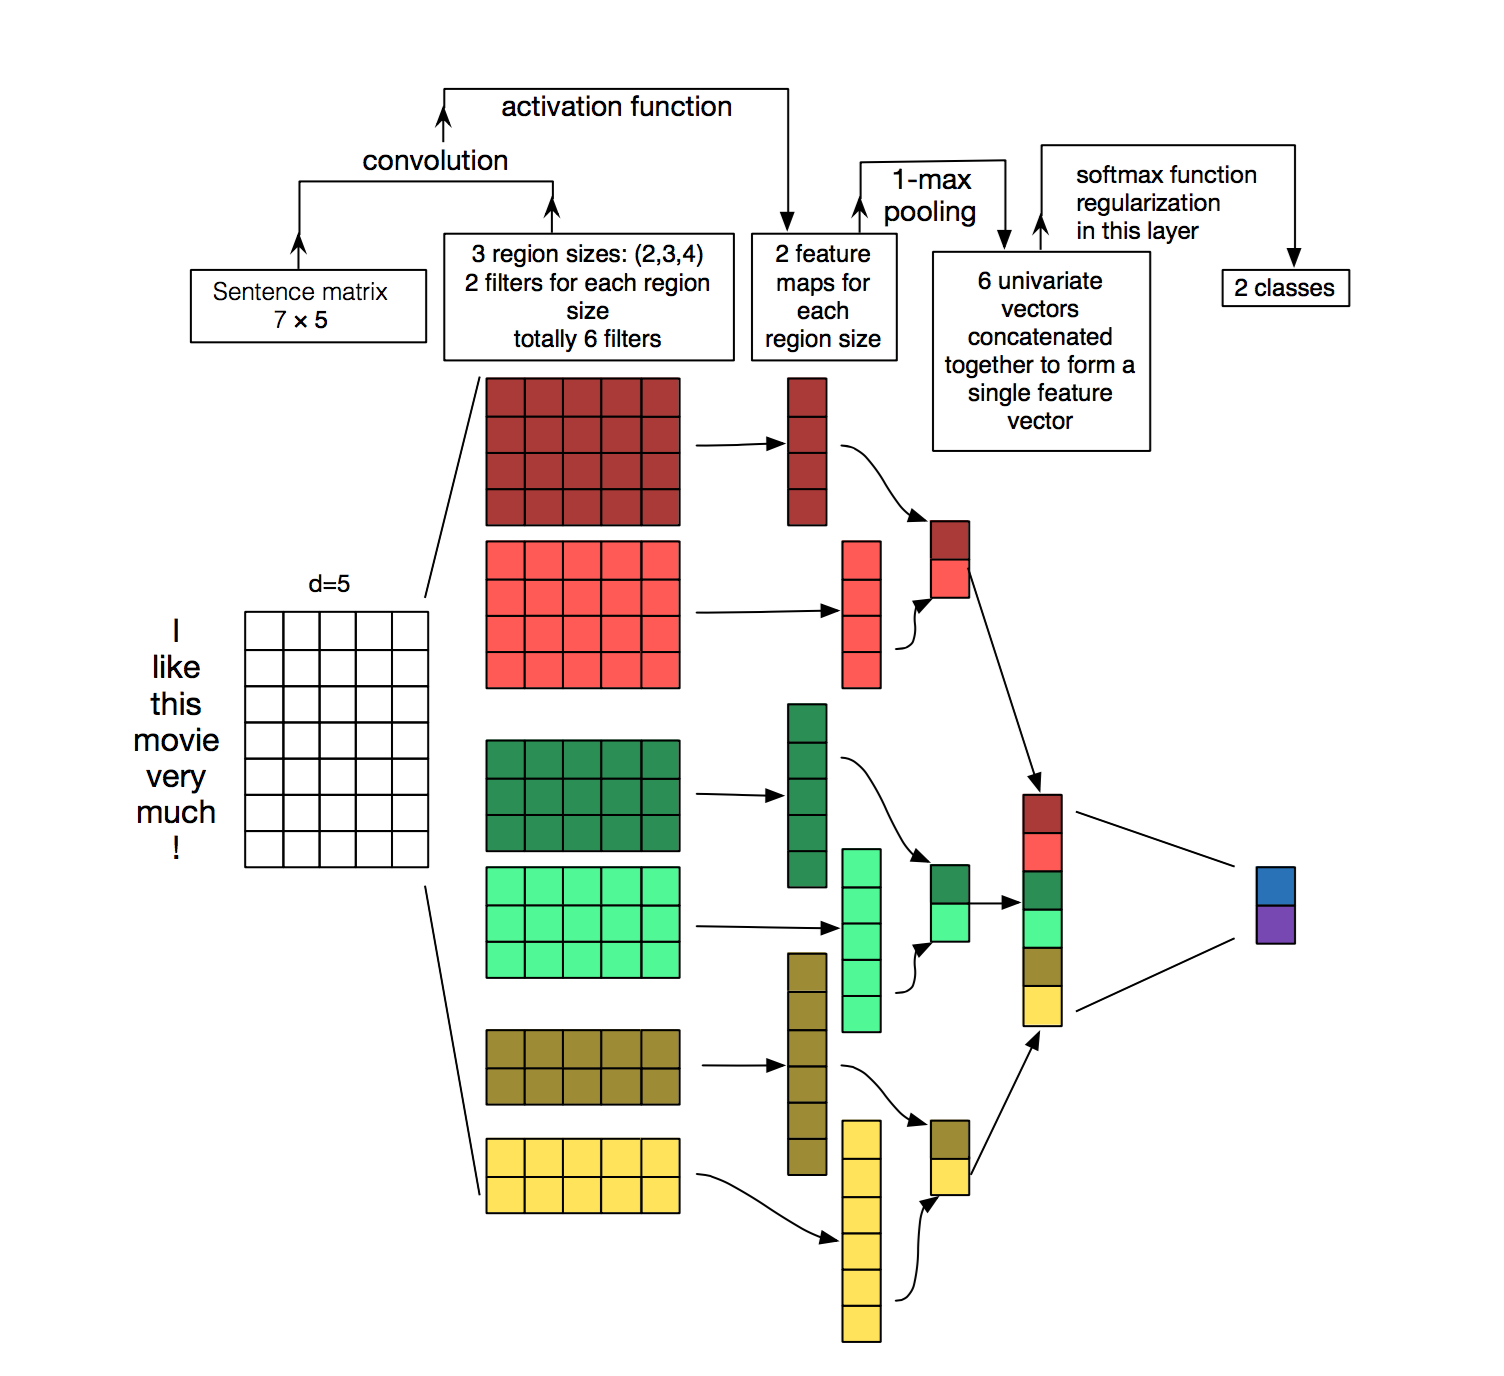
\includegraphics[width=.75\columnwidth]{kim_cnn}
\caption{\cite{zhang2015sensitivity} Illustration of a Convolutional Neural Network (CNN) architecture for sentence classification}
\label{fig:kim}
\end{figure}

\subsubsection{Recurrent neural network.}
Long Short Term Memory (LSTM) and Bidirectional LSTM are types of Recurrent Neural Network (RNN) aiming at capture dynamic temporal behaviour.
This behaviour suggest us to use them for the stance detection, in particular we use straightforward architectures made of an embedded input layer followed by an LSTM layer of 128 units, terminated by a dense layer for both normal and bidirectional models.